% Parte 2: Desagregação e Virtualização
\section{Desagregação e Virtualização}

\begin{frame}{Redes Tradicionais vs Virtualizadas}
\begin{itemize}
  \item \textbf{Antes:} nas redes legadas, o hardware (roteadores, switches, firewalls) era projetado de forma proprietária, com software integrado e fechado.  
  \item \textbf{Agora:} as funções de rede foram desacopladas e podem rodar em servidores COTS (\textit{Commercial Off-The-Shelf}), equipamentos comuns de TI, o que reduz custos e aumenta a flexibilidade.  
  \item \textbf{Exemplo ilustrativo:} antes era como comprar um aparelho “tudo em um”; agora é possível usar peças modulares conectadas, escolhendo cada componente de acordo com a necessidade.  
\end{itemize}
\end{frame}

\begin{frame}{Tecnologias Habilitadoras}
\begin{itemize}
  \item \textbf{NFV (\textit{Network Functions Virtualization}):} permite que funções como firewall, load balancer ou EPC (núcleo de rede 4G/5G) sejam executadas em máquinas virtuais ou containers.  
  \item \textbf{SDN (\textit{Software Defined Networking}):} separa o plano de controle (decisões sobre como rotear pacotes) do plano de dados (encaminhamento físico).  
  \item \textbf{Benefícios combinados:} mais automação, facilidade de escalar serviços e redução de CAPEX/OPEX.  
  \item \textbf{Analogia:} NFV é como instalar diferentes aplicativos em um mesmo computador, e SDN é como ter um “sistema operacional central” que coordena todos eles.  
\end{itemize}
\end{frame}

\begin{frame}
    \frametitle{Virtualização das Funções de Rede (NFV)}
    \begin{itemize}
        \item \textbf{Definição}: Abstração das funções de rede do hardware proprietário, executando-as em ambiente virtualizado.
        \item \textbf{Componentes Principais}: VNF (Funções de Rede Virtualizadas), NFVI (Infraestrutura de Virtualização).
        \item \textbf{Vantagens}: Redução de custos, flexibilidade, rapidez na introdução de serviços.
    \end{itemize}
\end{frame}

\begin{frame}
    \frametitle{Arquitetura NFV}
    \begin{itemize}
        \item \textbf{Virtualização do EPC (\textit{Evolved Packet Core})}: Gestão centralizada e flexível do core da rede.
        \item \textbf{vRAN (\textit{Virtualized Radio Access Network})}: Otimização da rede de acesso rádio.
        \item \textbf{\textit{Edge Computing}}: Suporte a aplicações de baixa latência e alta demanda.
    \end{itemize}
    \begin{figure}
        \centering
        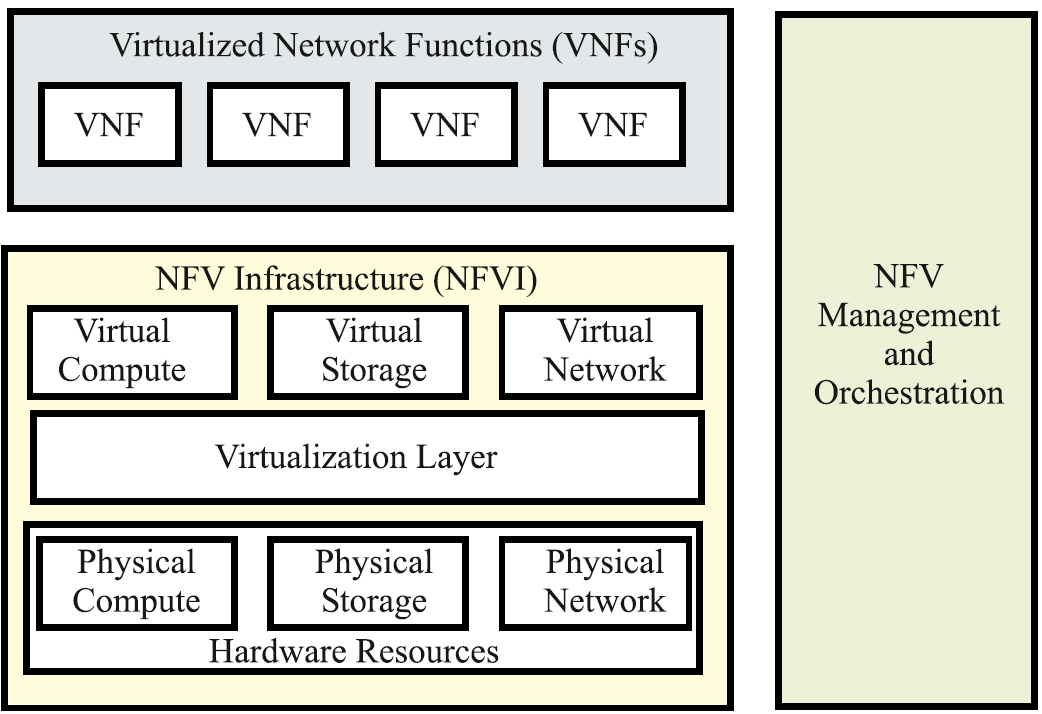
\includegraphics[width=0.45\linewidth]{figs/ArquiteturaNFV.png}
        \caption{Arquitetura geral NFV\footcite{NFV_architecture}}
    \end{figure}
\end{frame}

\begin{frame}{Redes Definidas por Software (SDN)}
    \begin{itemize}
        \item \textbf{Definição}: Arquitetura de rede que separa o plano de controle do plano de dados.
        \item \textbf{Componentes Principais}: Aplicações de rede, controlador SDN, switches programáveis, interfaces.
        \item \textbf{Vantagens}: Flexibilidade, centralização do controle, automação.
    \end{itemize}
    \begin{figure}
        \centering
        \subfloat[Tradicional]{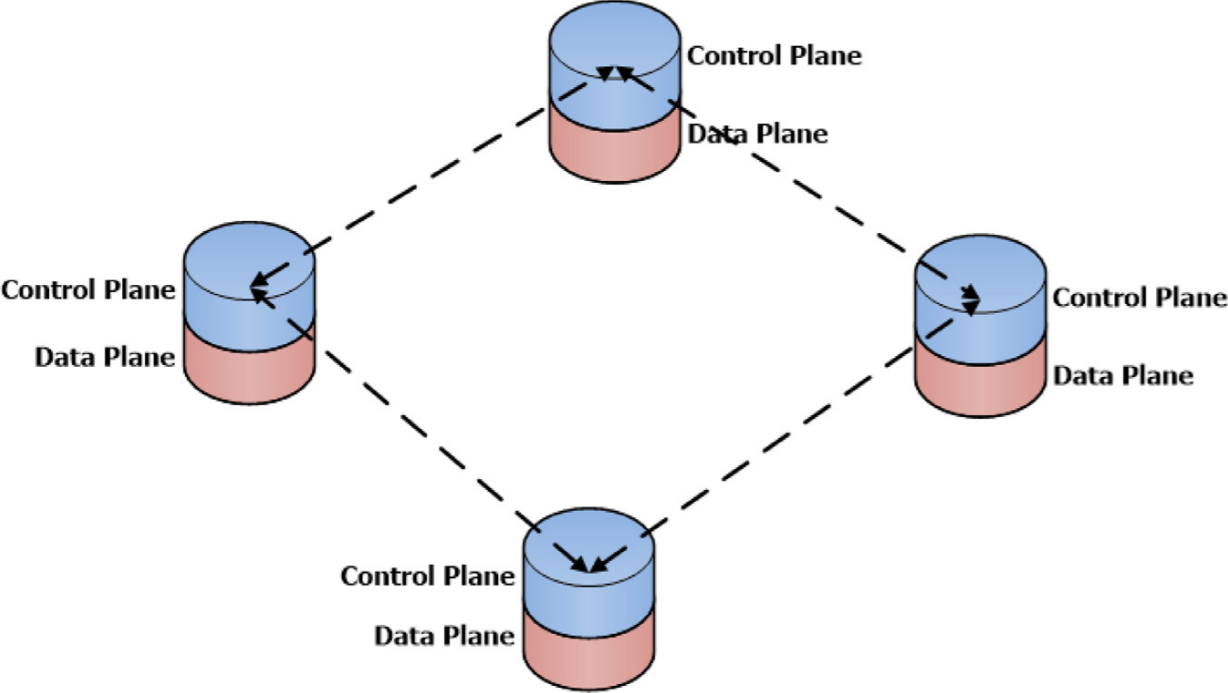
\includegraphics[width=0.45\linewidth]{figs/rede_tradicional.png}}\qquad
        \subfloat[SDN]{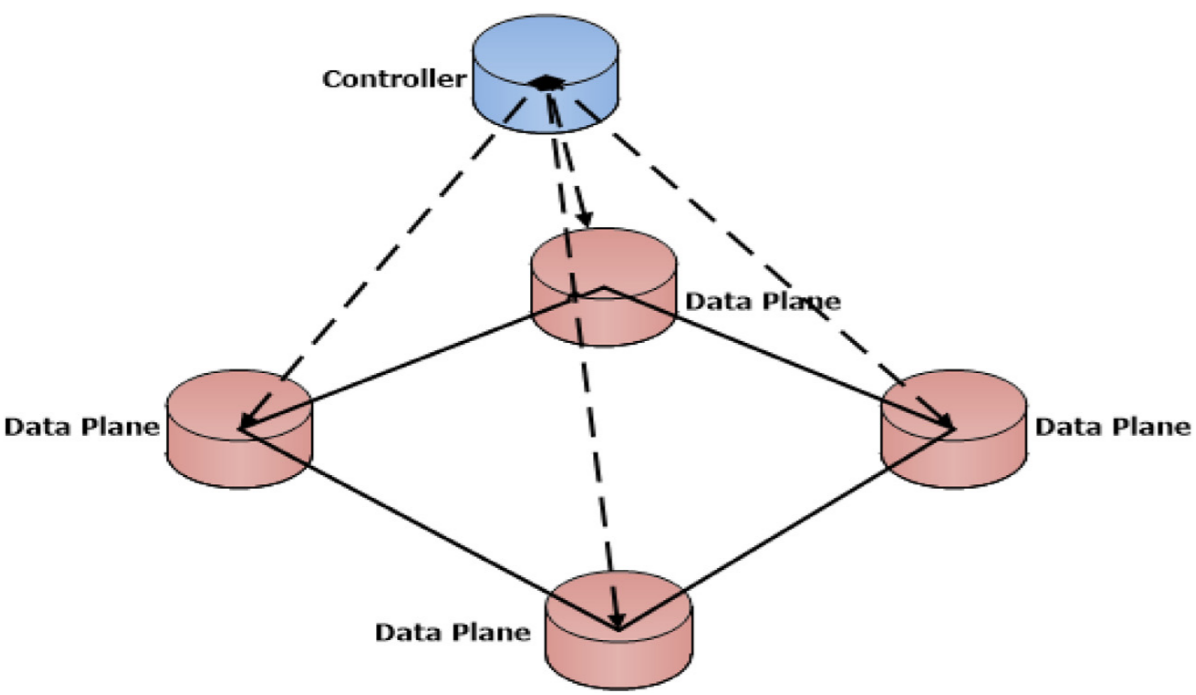
\includegraphics[width=0.45\linewidth]{figs/rede_sdn.png}}
        \caption{Redes tradicionais vs SDN\footcite{Plane_Separation}}
        \end{figure}
\end{frame}

\begin{frame}{Arquitetura SDN}
    \begin{columns}
        \begin{column}{0.55\textwidth}
            \begin{itemize}
                \item \textbf{Plano de Aplicação}: Controle dos recursos via programação.
                \item \textbf{Plano de Controle}: Gerência centralizada dos recursos de rede.
                \item \textbf{Plano de Dados}: Dispositivos de comutação físicos ou virtuais.
                \item \textbf{Interfaces}: Comunicação entre os planos, ao norte (REST), sul (OpenFlow, P4), leste, oeste (API dos controladores).
        \end{itemize}            
        \end{column}
        \begin{column}{0.45\textwidth}
            \vspace{1cm}
            \begin{figure}[h]
                \centering
                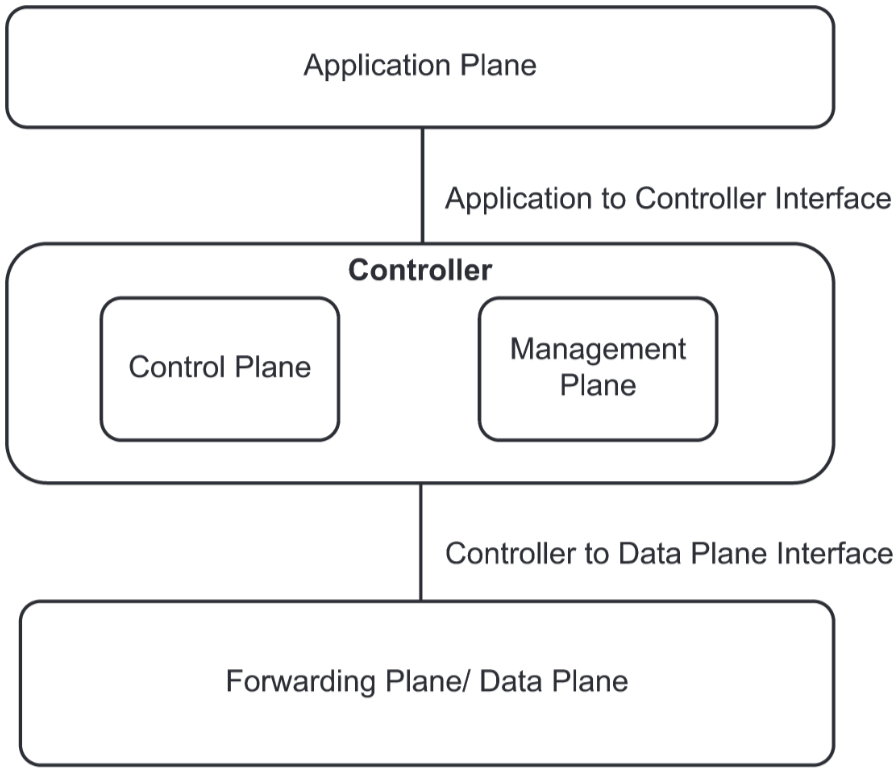
\includegraphics[width=\textwidth]{figs/SDN_arquitetura.png}
                \caption{Arquitetura SDN\footcite{Recommended_SDN_Wireless}}
            \end{figure}
        \end{column}
    \end{columns}
\end{frame}

\begin{frame}{Fatiamento de Rede (\textit{Network Slicing})}
    \begin{itemize}
        \item \textbf{Definição}: Técnica que permite a criação de múltiplas redes virtuais independentes sobre uma única infraestrutura física, otimizadas para atender diferentes requisitos de serviços e aplicações dentro de uma rede 5G.
        \item \textbf{Componentes Principais}: NFV e SDN.
        \item \textbf{Vantagens}: Garantir QoS, agilidade de implantação, personalizar e otimizar recursos de rede para diferentes serviços.
    \end{itemize}
\end{frame}

\begin{frame}{Integração com Operadores de Telecom}
    \begin{figure}[h]
        \centering
        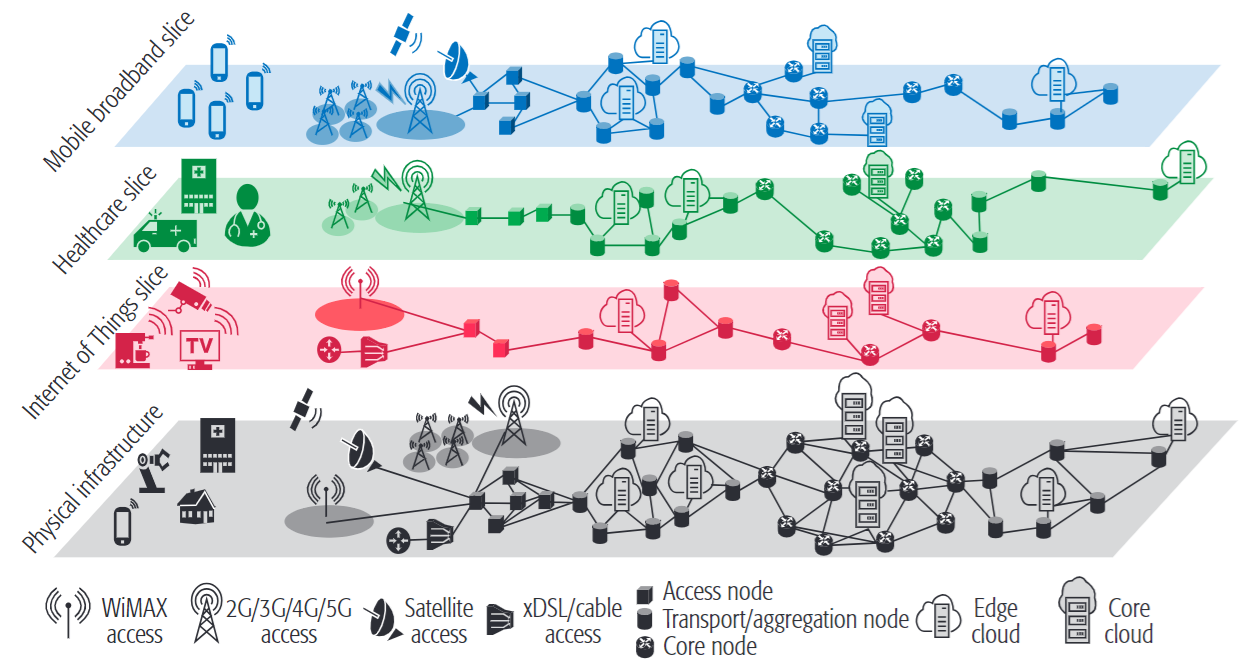
\includegraphics[width=\textwidth]{figs/Network_Slicing.png}
        \caption{Fatiamento de redes\footcite{Network_Slicing}}
    \end{figure}
\end{frame}

\begin{frame}{Desagregação em Telecom}
\begin{itemize}
  \item \textbf{Separação de funções:} no 5G, a RAN (Rede de Acesso Rádio) é dividida em RU (unidade de rádio), DU (unidade distribuída) e CU (unidade centralizada).  
  \item \textbf{Interfaces abertas:} definidas por padrões (ex.: eCPRI, F1, E2), permitem interoperabilidade entre equipamentos de diferentes fornecedores.  
  \item \textbf{Impacto:} facilita a entrada de novos \textit{players} e aumenta a competitividade no mercado.  
  \item \textbf{Exemplo:} uma operadora pode usar a RU da Nokia, a DU da Intel e a CU da Ericsson, todos integrados por interfaces abertas.  
\end{itemize}
\end{frame}

\begin{frame}{Benefícios da Desagregação}
\small
\begin{itemize}
  \item \textbf{Separação hardware/software} $\rightarrow$ menor dependência de fornecedores proprietários.
  \item \textbf{Arquitetura modular (RU, DU, CU)} $\rightarrow$ flexibilidade na evolução e no dimensionamento da rede.
  \item \textbf{Interfaces abertas/padronizadas} (3GPP, O-RAN, ETSI) $\rightarrow$ interoperabilidade real.
  \item \textbf{Ambiente multifornecedor} $\rightarrow$ redução de custos e aumento da concorrência.
  \item \textbf{Escalabilidade seletiva} $\rightarrow$ expande apenas o módulo necessário (otimiza CAPEX/OPEX).
  \item \textbf{Automação e programabilidade} (SDN, APIs) $\rightarrow$ gestão centralizada e operações mais inteligentes.
  \item \textbf{Inovação acelerada} $\rightarrow$ entrada de novos \textit{players} e serviços lançados mais rapidamente.
\end{itemize}
\end{frame}
